\documentclass[letterpaper,12pt]{article}
\usepackage{tabularx,amsmath,graphicx}
\usepackage[margin=1in,letterpaper]{geometry}
\usepackage{cite}
\usepackage[final]{hyperref}
\hypersetup{
colorlinks=true,
linkcolor=blue,
citecolor=blue,
filecolor=magenta,
urlcolor=blue         
}
\begin{document}
\title{WES268A Fall 2015 \\ Digital Communications \\ Lab 1: Prelab}
\author{Joshua Emele $<$jemele@acm.org$>$}
\maketitle

\section{Theory Problems}

\subsection{Spectrum of AM modulated signals}
\begin{figure}[hbtp]
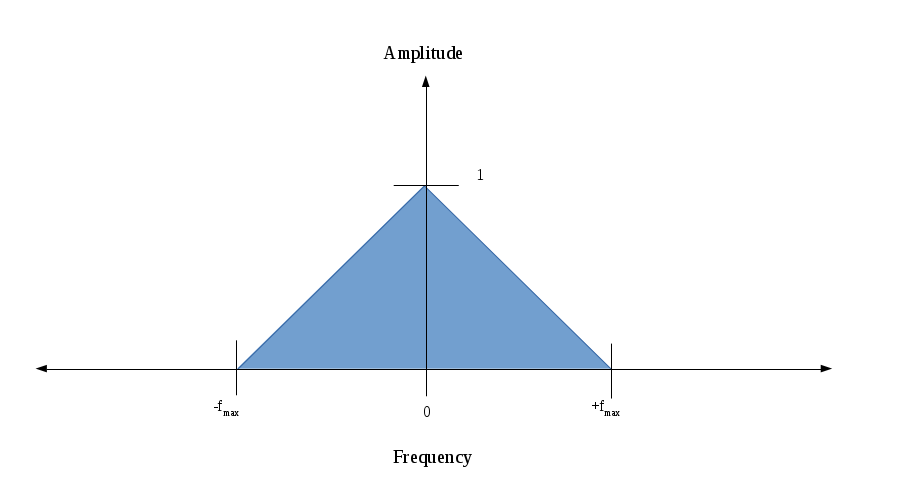
\includegraphics[width=0.6\columnwidth]{prelab1-figure1}
\caption{
\label{fig:prelab1-figure1}
{\bf A sketch of the frequency spectrum of the baseband signal $S(f)$.
}
}
\end{figure}

\begin{figure}[hbtp]
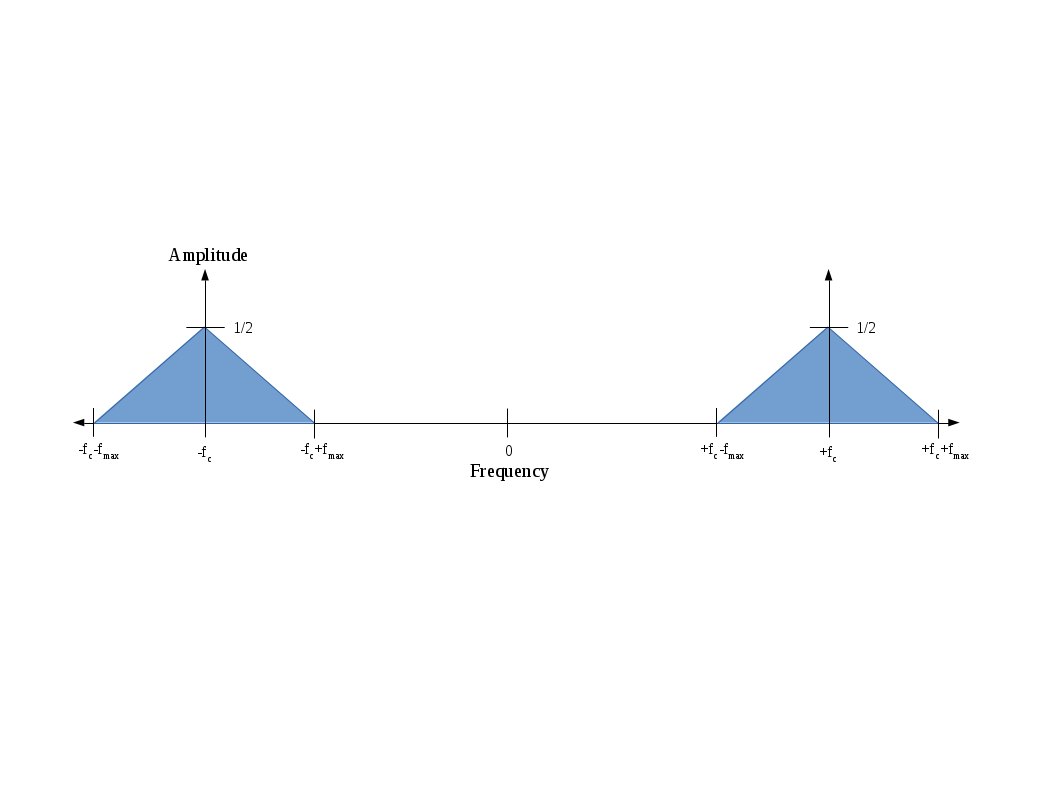
\includegraphics[width=1.0\columnwidth]{prelab1-figure1a}
\caption{
\label{fig:prelab1-figure1a}
{\bf A sketch of the frequency spectrum of the amplitude-modulated passband
signal $\tilde{S}(f)$.
}
}
\end{figure}

\begin{figure}[hbtp]
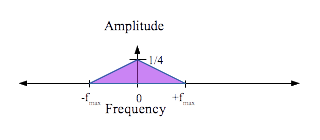
\includegraphics[width=1.0\columnwidth]{prelab1-figure1b}
\caption{
\label{fig:prelab1-figure1b}
{\bf A sketch of the frequency spectrum of the demodulated signal.
}
}
\end{figure}
\pagebreak

\subsection{Frequency demodulation errors}

\begin{figure}[hbtp]
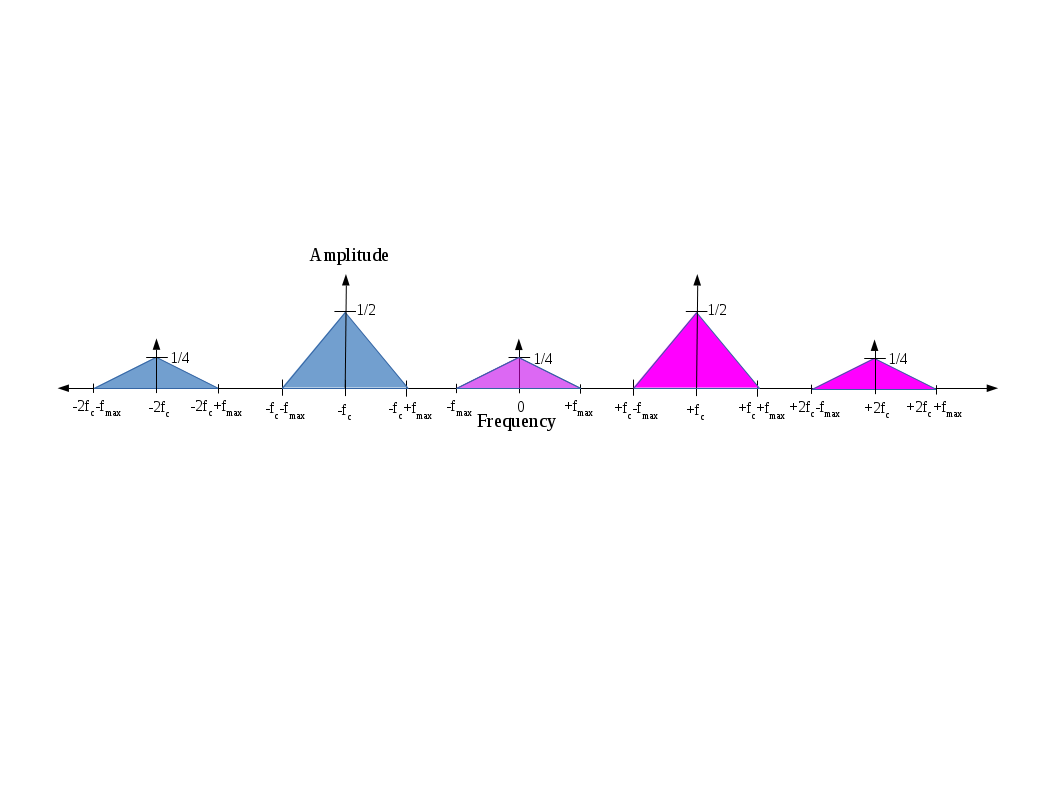
\includegraphics[width=1.0\columnwidth]{prelab1-figure2a}
\caption{
\label{fig:prelab1-figure2a}
{\bf A sketch of the frequency spectrum of the demodulated signal with
frequency error $x=0$.
}
}
\end{figure}

As frequency error is introduced, the aliased baseband copies shift past each
other.  Because $f_{c}$ dominates $f_{max}$, we assume $f_{c}$ is at least
several orders of magnitude larger than $f_{max}$.

\begin{figure}[hbtp]
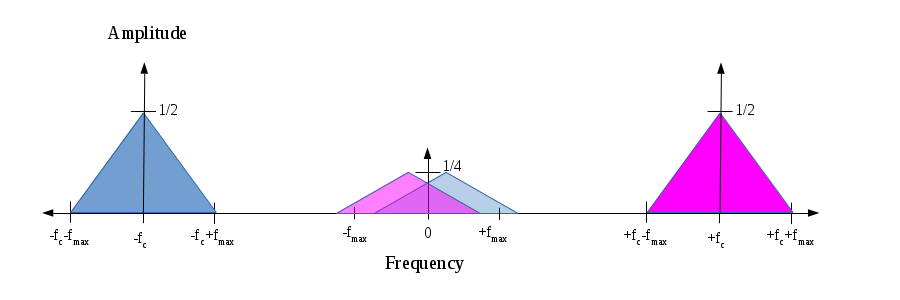
\includegraphics[width=1.0\columnwidth]{prelab1-figure2b}
\caption{
\label{fig:prelab1-figure2b}
{\bf A sketch of the frequency spectrum of the demodulated signal with
frequency error $x=\frac{f_{max}}{10f_{c}}$. Note that spectral copies at
$\pm2f_{c}$ exist but are not visible in the figure.
}
}
\end{figure}

\begin{figure}[hbtp]
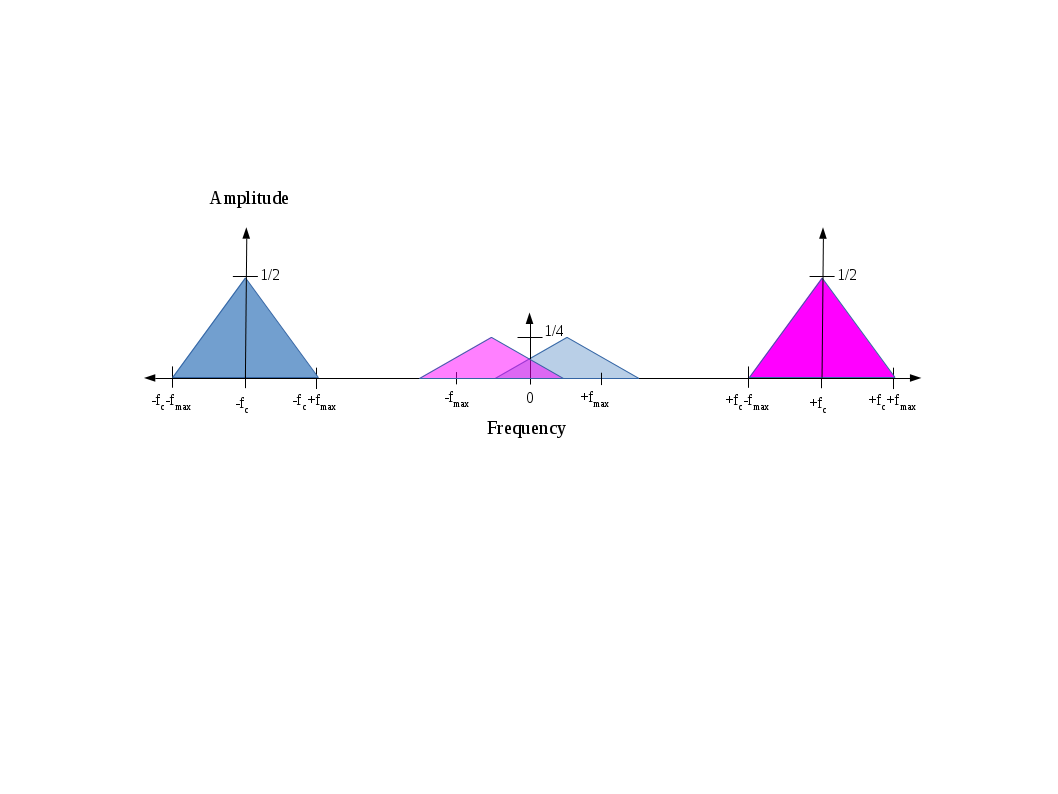
\includegraphics[width=1.0\columnwidth]{prelab1-figure2c}
\caption{
\label{fig:prelab1-figure2c}
{\bf  A sketch of the frequency spectrum of the demodulated signal with
frequency error $x=\frac{f_{max}}{f_{c}}$.  Note that spectral copies at
$\pm2f_{c}$ exist but are not visible in the figure.
}
}
\end{figure}

The frequency error is now a magnitude larger than before, but is still
relatively small because $f_{c}$ is several order of magnitude larger than
$f_{max}$. Even as the aliased copies slide past each other at baseband with
the introduction of frequency error, the Nyquist rate of the baseband signal is
unaffected because $f_{max}$ remains unchanged.
\pagebreak

\subsection{Phase demodulation errors}

An AM signal $\tilde{s}(t)=A\ cos(2 \pi f_{c}t)$ where $A$ is a constant is
demodulated by $cos(2 \pi f_{c}t+\phi)$ where $\phi$ represents a phase error.

An expression for the demodulated signal $d(t,\phi)$ as a function of the phase
error $\phi$ is given by:
\begin{equation}
d(t,\phi)=A\ cos(2 \pi f_{c}t)cos(2 \pi f_{c}t+\phi)
\end{equation}

The period of the carrier $f_{c}$ is given by $T=\frac{1}{f_{c}}$.

If the demodulated signal $d(t,\phi)$ is integrated over a time period $T$ that
is many times the period of the carrier (i.e., $N\ T$, where $N >= 2$), the value
of the integral without phase error ($\phi=0$) is given by:

\begin{equation}
\begin{split}
M_{0} & = \int_{0}^{\frac{2}{f}}A\ cos(2\pi f_{c}t)cos(2\pi f_{c}t) \\
 & = \frac{1}{f}
\end{split}
\end{equation}

The value of the integral with phase error ($\phi\neq0$) over the same period is
given by:

\begin{equation}
\begin{split}
M_{1} & = \int_{0}^{\frac{2}{f}}A\ cos(2\pi f_{c}t)cos(2\pi f_{c}t+\phi) \\
 & = \frac{cos(\phi)}{f}
\end{split}
\end{equation}

The maximum phase error $\phi$ that can be tolerated for the demodulated signal
to ensure the amplitude is within ten percent of the amplitude without a phase
error is given by:

\begin{equation}
\begin{split}
\frac{M_{0}}{M_{1}}\leq10 \\
sec(\phi)\leq10 \\
|\phi|\leq\ sec^{-1}(10) \\
|\phi|\leq\ 0.4706 \\
\end{split}
\end{equation}

\subsection{Agilent tutorial on Spectrum Analyzers}

The resolution bandwidth required to resolve signals separated by 50 kHz that
differ by 40 dB in power is given by:

\begin{equation}
-40\ log_{10}\left(\left(\frac{50000}{\frac{B}{2\sqrt{\sqrt[4]{2}-1}}}\right)^2 - 1\right) = -40\ dB
\end{equation}

\begin{figure}[hbtp]
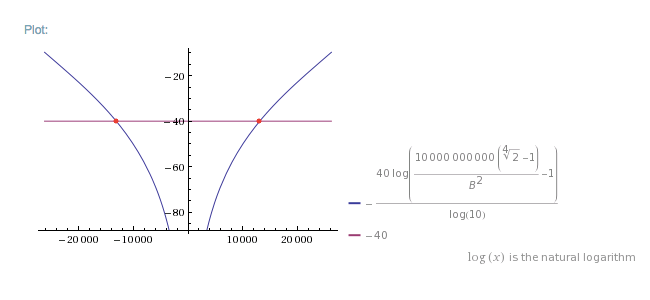
\includegraphics[width=1.0\columnwidth]{prelab1-figure4}
\caption{
\label{fig:prelab1-figure4}
{\bf Calculating the resolution bandwidth that meets design specifications.
}
}
\end{figure}

Solving for the resolution bandwidth $B\approx13115\ Hz$.

Changing the video bandwidth (filter) or averaging will affect the result. If
the video bandwidth is changed, the resolution bandwidth will also need to
change. Averaging acts as low-frequency filter that rejects high frequency
noise, effectively smoothing the signal. This reduction in noise will also
affect the required resolution bandwidth.

The expected value of additive noise is zero – averaging acts a low-pass filter
that smooths the signal and eliminates the additive noise. This reduction in
noise will affect the required resolution
bandwidth.
\pagebreak

\section{Matlab/Simulink Simulations}

\begin{figure}[hbtp]
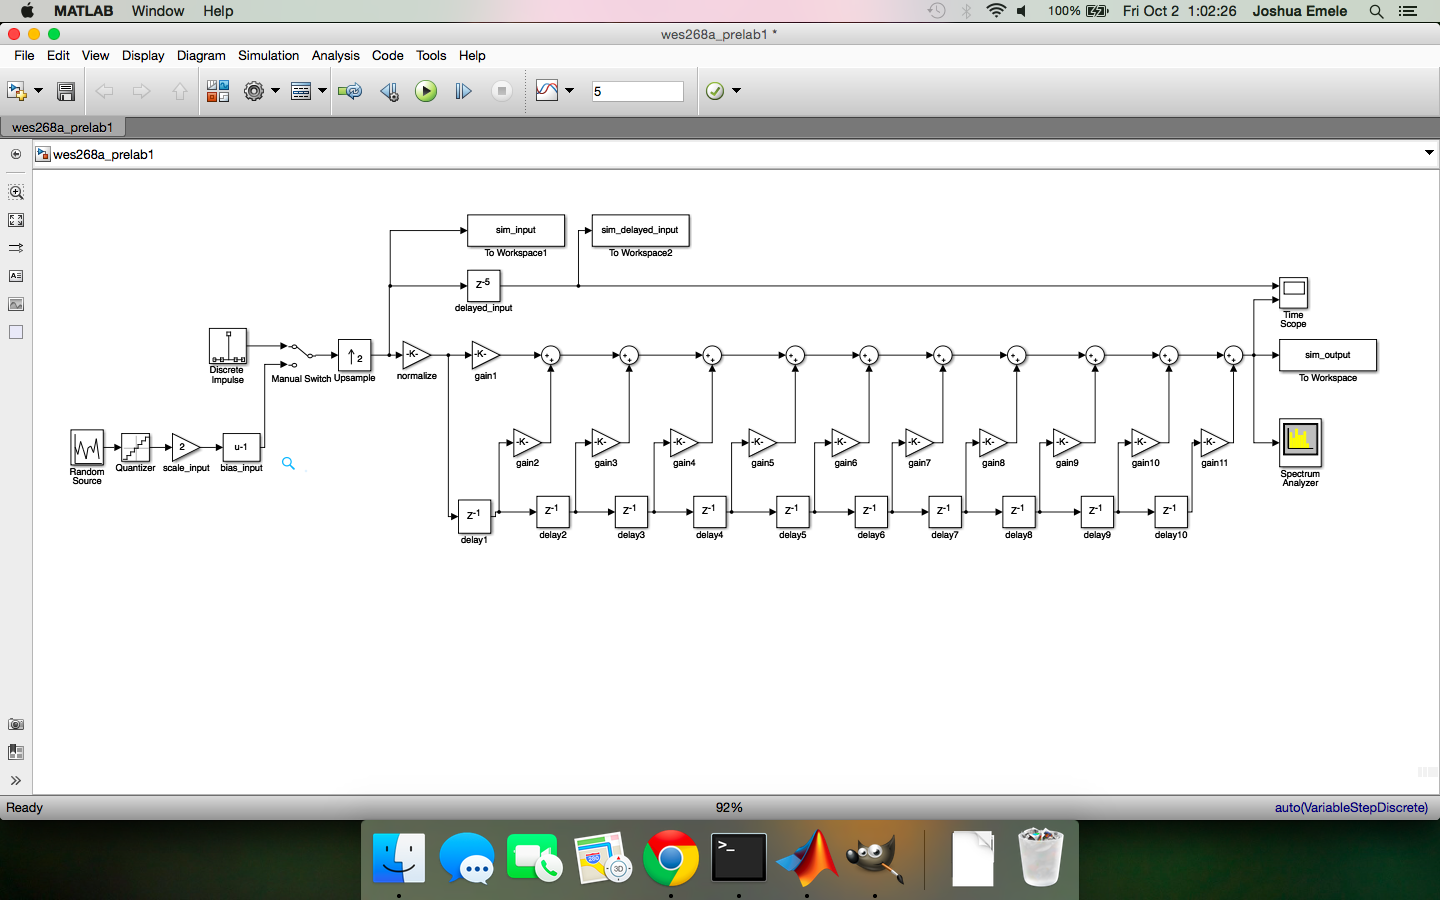
\includegraphics[width=1.0\columnwidth]{prelab1-simulation-diagram}
\caption{
\label{fig:prelab1-simulation-diagram}
{\bf A simulink model that implements a raised cosine pulse with $\beta=0.5$,
$delay = 5\ samples$, and $rate = 2\ samples/symbol$. A switch is provided to
toggle between measuring the filter's impulse response and the filter response
to modulated symbol data. An upsample block is provided to achieve the required
sample rate.
}
}
\end{figure}

\begin{figure}[hbtp]
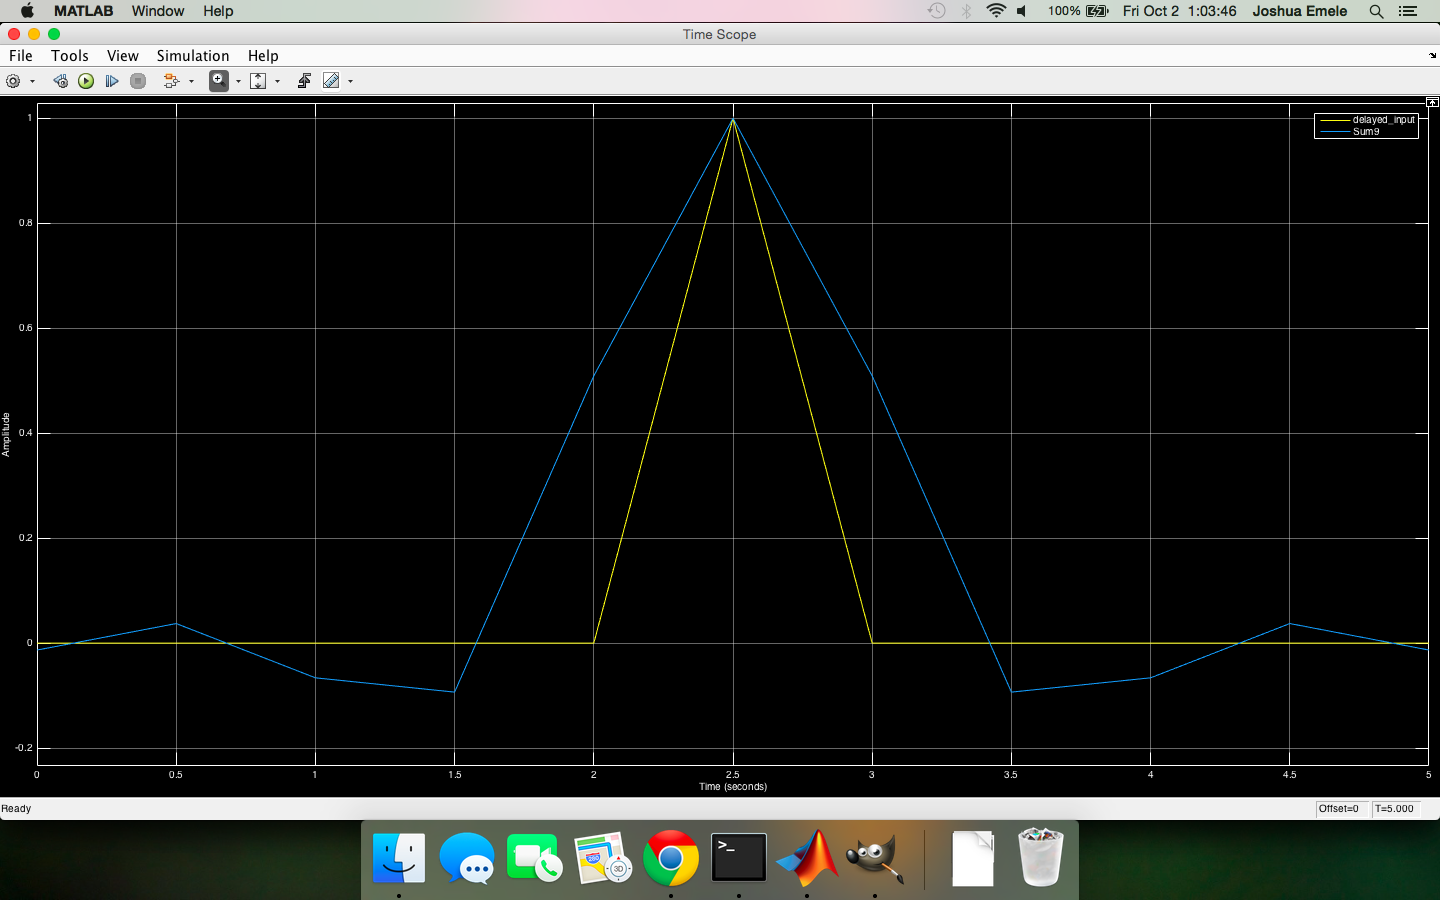
\includegraphics[width=1.0\columnwidth]{prelab1-filter-impulse-response}
\caption{
\label{fig:prelab1-filter-impulse-response}
{\bf The filter impulse response.
}
}
\end{figure}

\begin{figure}[hbtp]
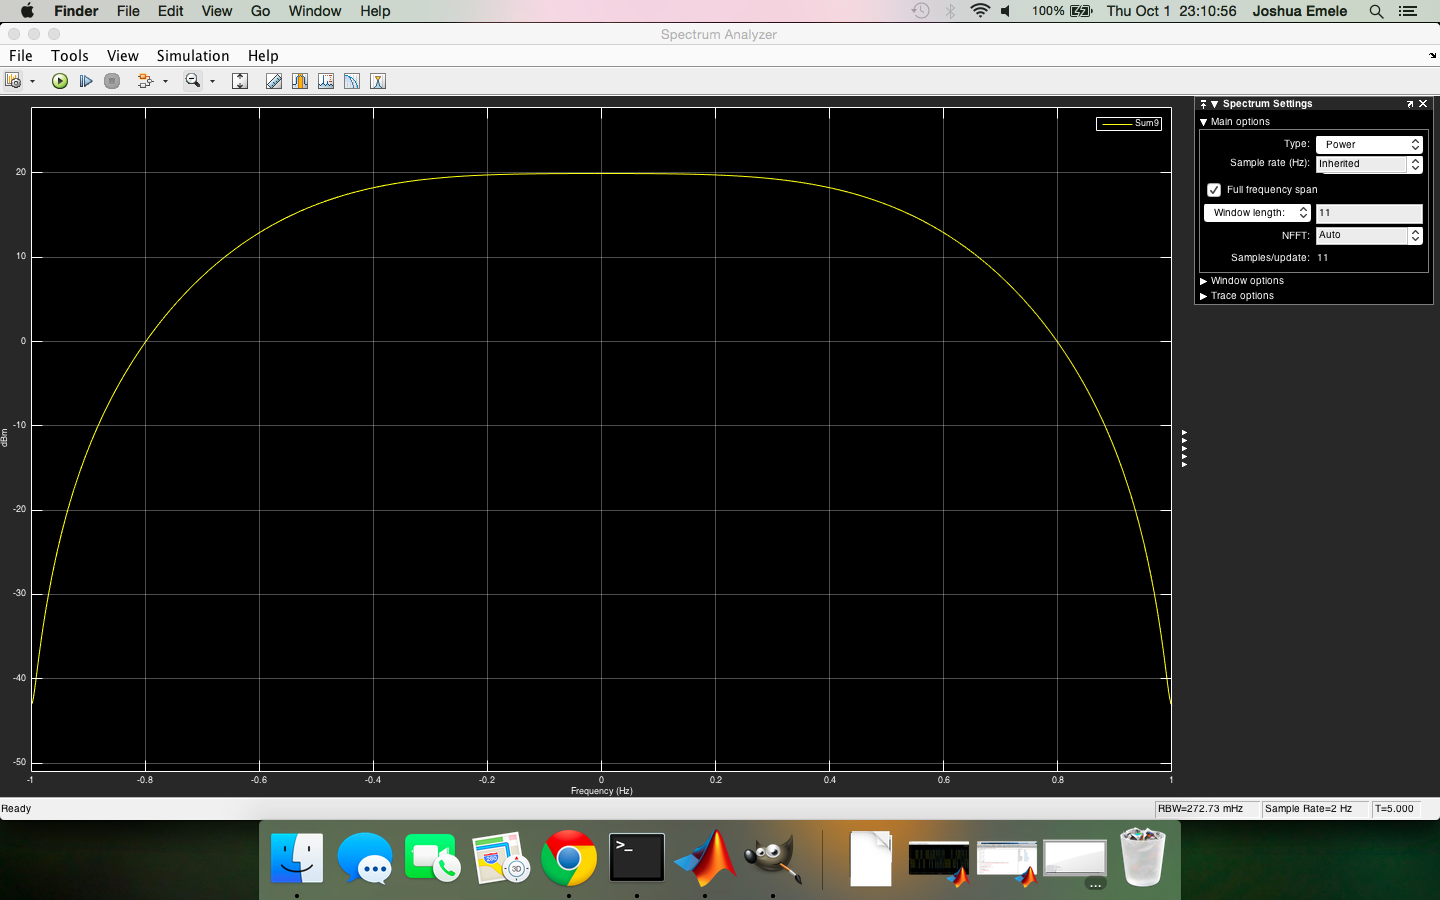
\includegraphics[width=1.0\columnwidth]{prelab1-filter-impulse-spectrum}
\caption{
\label{fig:prelab1-filter-impulse-spectrum}
{\bf The filter frequency response.
}
}
\end{figure}

\begin{figure}[hbtp]
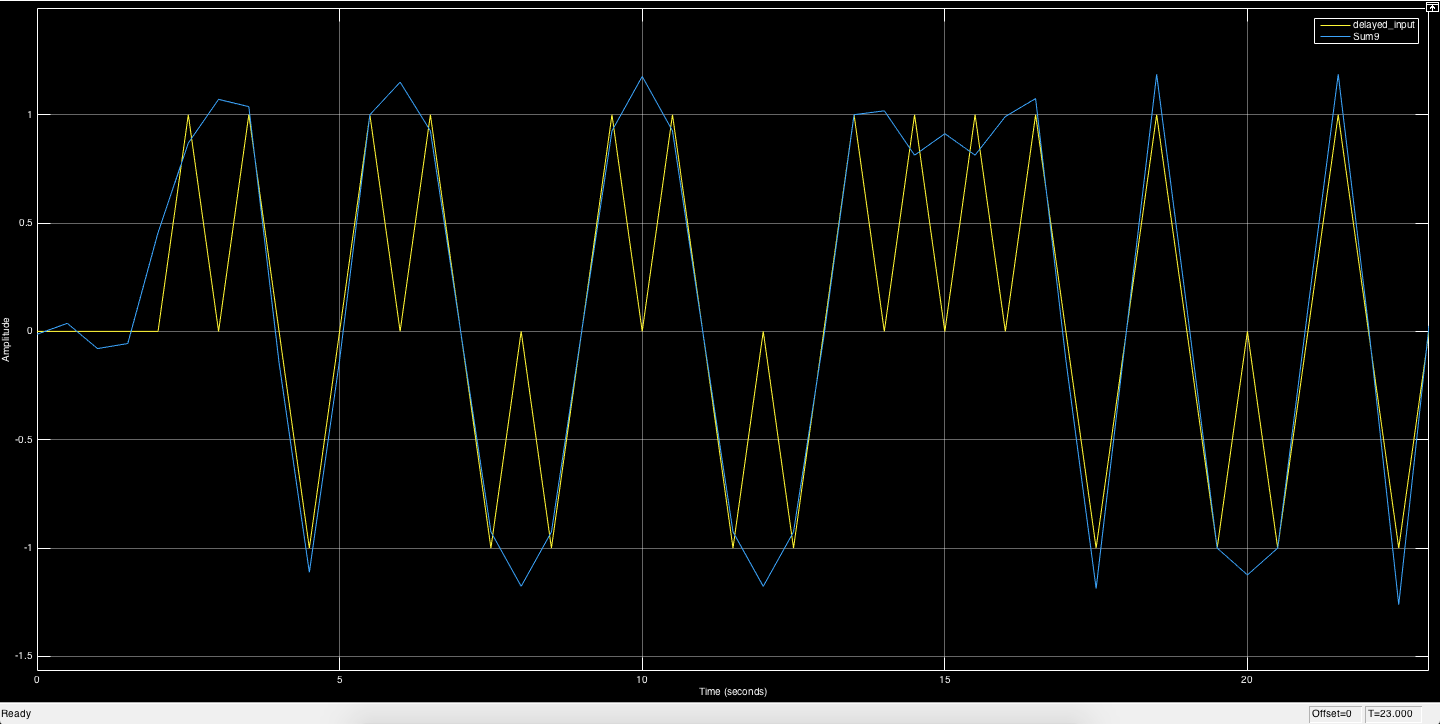
\includegraphics[width=1.0\columnwidth]{prelab1-filter-input-output}
\caption{
\label{fig:prelab1-filter-input-output}
{\bf The filter input and output for at least 20 symbols of upsampled data.
}
}
\end{figure}

\begin{figure}[hbtp]
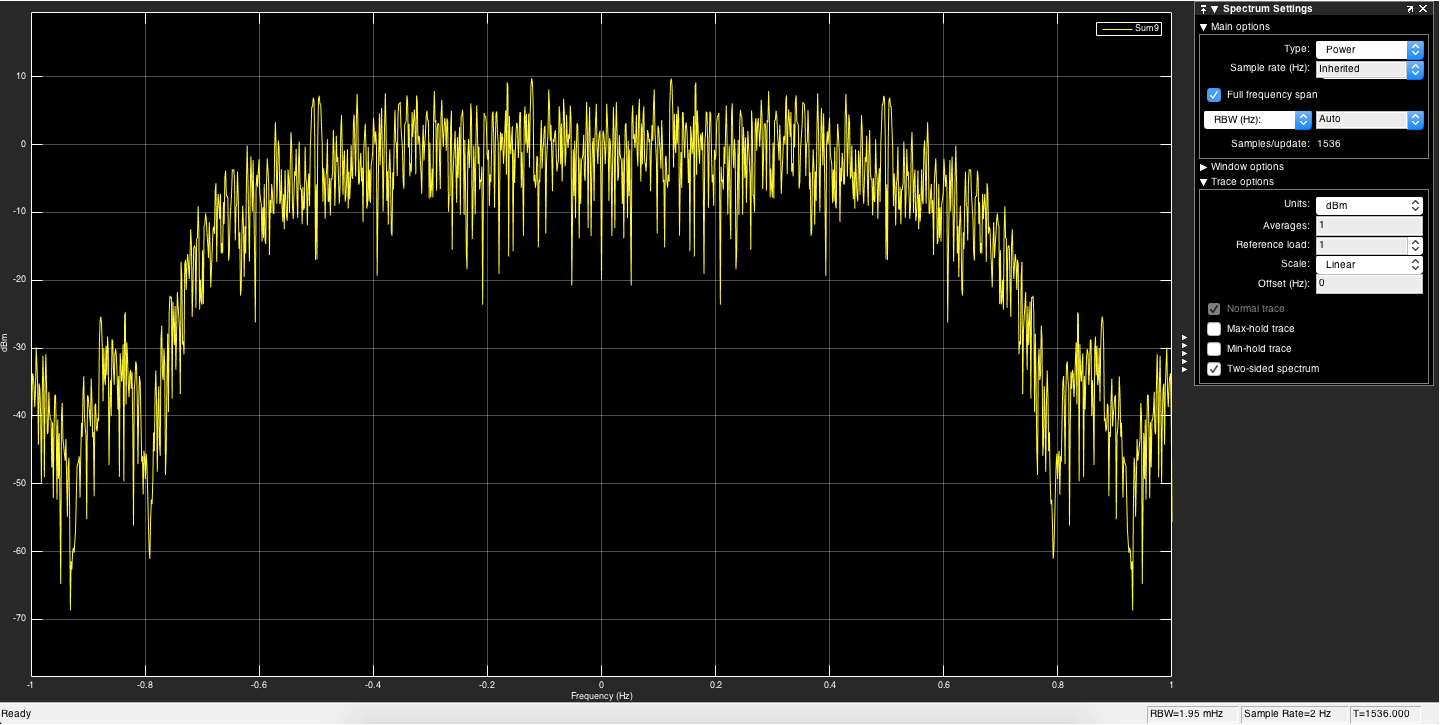
\includegraphics[width=1.0\columnwidth]{prelab1-filter-output-spectrum}
\caption{
\label{fig:prelab1-filter-output-spectrum}
{\bf The filter output spectrum for modulated BPSK data. The spectrum looks
like a windowed function.
}
}
\end{figure}



\end{document}
